% standalone wrapper for a tikz picture
\documentclass[tikz,border=2pt]{standalone}
\usepackage{xcolor}
\usepackage{tikz}
\usetikzlibrary{shapes,arrows,positioning,shadows,patterns,arrows.meta,calc}
\definecolor{cwAlert}{RGB}{220,50,50}
\definecolor{cwFlow}{RGB}{50,120,220}
\definecolor{cwDecoy}{RGB}{120,180,50}
\definecolor{cwBorder}{RGB}{80,80,80}
\definecolor{ImperialBlue}{RGB}{0,62,116}
\definecolor{ImperialNavy}{RGB}{0,33,71}
\definecolor{ImperialLightBlue}{RGB}{155,203,235}
\begin{document}

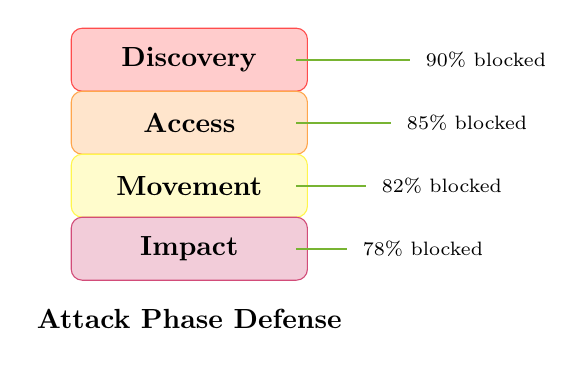
\begin{tikzpicture}[scale=0.8]
    % MITRE ATT&CK phases
    \node[draw=red!70, fill=red!20, rounded corners, minimum width=3cm, minimum height=0.8cm] at (0,3) {\textbf{Discovery}};
    \node[draw=orange!70, fill=orange!20, rounded corners, minimum width=3cm, minimum height=0.8cm] at (0,2) {\textbf{Access}};
    \node[draw=yellow!70, fill=yellow!20, rounded corners, minimum width=3cm, minimum height=0.8cm] at (0,1) {\textbf{Movement}};
    \node[draw=purple!70, fill=purple!20, rounded corners, minimum width=3cm, minimum height=0.8cm] at (0,0) {\textbf{Impact}};
    
    % Defense effectiveness
    \draw[thick, cwDecoy] (1.7,3) -- (3.5,3);
    \draw[thick, cwDecoy] (1.7,2) -- (3.2,2);
    \draw[thick, cwDecoy] (1.7,1) -- (2.8,1);
    \draw[thick, cwDecoy] (1.7,0) -- (2.5,0);
    
    \node[right] at (3.6,3) {\scriptsize 90\% blocked};
    \node[right] at (3.3,2) {\scriptsize 85\% blocked};
    \node[right] at (2.9,1) {\scriptsize 82\% blocked};
    \node[right] at (2.6,0) {\scriptsize 78\% blocked};
    
    \node[below] at (0,-0.8) {\textbf{Attack Phase Defense}};
\end{tikzpicture}
\end{document}
